% I am sure you have heard of few functions and used them in your daily life. For example, the function $f(x) = x^2$ is a function that takes a number and returns its square. Before defining a function, let us examine the known one like $f(x)=x^2$, it takes an input $x$ and returns an output $x^2$. If we input $2$ to the function, it returns $2^2=4$. If we input $3$, it returns $3^2=9$. If we again put the value $x=2$ it will return $2^2=4$ only not different value. That means the function $f(x)=x^2$ is a rule that assigns a unique output to each input.

% \section*{The Story of the Squaring Function}
\addcontentsline{toc}{subsection}{Introduction}
I'm sure you have encountered a few functions and used them in your daily life, even if you didn't realize it. Let's dive into the concept of functions with a familiar example: the function \( f(x) = x^2 \).\\

% \subsection*{The Story of the Squaring Box}

Imagine you have a magical box called the "Squaring Box." This box has a simple yet powerful rule: whatever number you put into it, it will square that number and give you the result.\\[2mm]


Let's see how this Squaring Box works with some examples:

\begin{itemize}
    \item \textsc{Input}: You put the number 2 into the Squaring Box.
    \begin{itemize}
        \item \textsc{Process}: The box squares the number (multiplies it by itself).
        \item \textsc{Output}: The box gives you \( 2^2 = 4 \).
    \end{itemize}
    
    \item \textsc{Input}: You put the number 3 into the Squaring Box.
    \begin{itemize}
        \item \textsc{Process}: The box squares this number.
        \item \textsc{Output}: The box gives you \( 3^2 = 9 \).
    \end{itemize}
    
    \item \textsc{Input}: You put the number 2 into the Squaring Box again.
    \begin{itemize}
        \item \textsc{Process}: The box squares the number.
        \item \textsc{Output}: The box gives you \( 2^2 = 4 \).
    \end{itemize}
\end{itemize}

Notice something important: every time you put the same number into the Squaring Box, you always get the same result. This consistency is what makes the Squaring Box special and reliable.


\begin{center}
    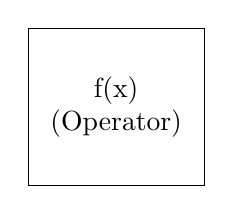
\begin{tikzpicture}
        \tikzstyle{block} = [rectangle, draw, text width=2cm, text centered, minimum height=2cm]
        \node[block] (box) at (0, 0){f(x)\\(Operator)};
        \tzline+[<-](box.west)(-1, 0){input}[l]
        \tzline+[->](box.east)(1, 0){output}[r]
    \end{tikzpicture}
\end{center}

\vbdefinition{We can define a function as a machine that takes an input, performs some process on that input (or sometimes does nothing), and then produces a unique output for every input.}

\addcontentsline{toc}{subsection}{Domain and Range}
\vbsubtitle{Domain and Range}
\begin{itemize}
    \item Sometimes domain is also referred as independent variable and range as dependent variable. 
    \item[*] Domain: \vbdefinition{Set of all possible inputs of any function for which it outputs a finite real number is called domain of that function.\\[2mm]
    For the above function $f(x)=x^2$ any real number can be inputted in this function will still output a finite real number. So, domain for this square function will be all real numbers. 
    \[ x \in (-\infty, ~+\infty) \]
    }
    \item[*] Range: \vbdefinition{Set of all possible outputs of any function is called range of that function.\\[2mm]
    For the function $f(x)=x^2$, it can output any positive number and zero. So range for this function will be all positive real numbers including zero. 
    \[ y \in [0, ~+\infty) \]
    }
\end{itemize}

\pagebreak

\addcontentsline{toc}{subsection}{Types of Functions}
\vbtitle{Naming of Functions}
\begin{enumerate}
    \addcontentsline{toc}{subsubsection}{Algebraic Functions} 
    \item Algebraic Functions: \vbdefinition{These are the functions consisting of finite number of terms involving  powers and radicals of the independent variable, constants and fundamental mathematical operations,  $+$, $-$, $\times$, $\div$.}
        \begin{enumerate}
            \item Polynomial Functions: \vbdefinition{A function of the form 
            \[ f(x) = a_0x^n + a_1x^{n-1} + \cdots + a_{n-1}x + a_n \]
            where $a_0$, $a_1$, $\cdots$, $a_n$ are real constants and $n$ is non-negative integer, is called a polynomial. If $a_0 \neq 0$, then $n$ is the degree of the polynomial.
            }
            \textbf{Examples:}
            \begin{align*}
                f(x) &= x^9 + 5x  &\text{Polynomial of degree $9$}\\
                g(x) &= x^2 + 3x -5  &\text{Polynomial of degree $2$}\\
                h(x) &= 7 = 7x^0  &\text{Polynomial of degree $0$}
            \end{align*}
            \item Fractional rational functions: \vbdefinition{It is defined as the ratio of two polynomials.}
            \begin{align*}
                \text{Let } P(x) &= a_n x^n + a_{n-1} x^{n-1} + \ldots + a_1 x + a_0, \\
                Q(x) &= b_m x^m + b_{m-1} x^{m-1} + \ldots + b_1 x + b_0,
                \end{align*}
                then \( f(x) = \frac{P(x)}{Q(x)} \) is a fractional rational function or simply we call it a rational function. The domain of a rational function is all real numbers except when the denominator is zero, i.e., \( Q(x) \neq 0 \).
                
                \textbf{Examples:}
                \[
                f(x) = \frac{x-3}{x-2} \quad \text{domain: } x \in \mathbb{R} - \{2\}.
                \]
                
            \item Irrational Functions: \vbdefinition{If in \( y = f(x) \), operations of addition, subtraction, multiplication, division, and raising to a power with non-integral rational exponents are performed on the right-hand side, the function \( y = f(x) \) is irrational.}
                
                \textbf{Examples:}
                \[
                f(x) = \sqrt{x} \quad ; \quad \frac{x^2 + \sqrt{x}}{\sqrt{1+3x^2}} \quad \text{etc.}
                \]
                
                \textbf{Note:} The three kinds of algebraic functions mentioned above don't cover all algebraic functions. An algebraic function is any function \( y = f(x) \) satisfying
                \[
                P_0(x)y^n + P_1(x)y^{n-1} + \ldots + P_{n-1}(x)y + P_n(x) = 0
                \]
                where \( P_0(x), P_1(x), \ldots, P_n(x) \) are certain polynomials in \( x \).
                
        \end{enumerate}

    \addcontentsline{toc}{subsubsection}{Transcendental Functions}
    \item Transcendental Functions: \vbdefinition{A transcendental function is a type of function that is not algebraic. In other words, a transcendental function cannot be expressed as a finite sequence of the algebraic operations of addition, subtraction, multiplication, division, and root extraction.}
        \begin{enumerate}
            \item Exponential Functions: \vbdefinition{
                The function \( f(x) = a^x, \, a > 0, \, a \neq 1 \) is called an exponential function. Here base ‘\( a \)’ is a constant.
            }
            \begin{center}
                \begin{tikzpicture}
                    \draw[->] (-4,0) -- (5,0) node[right] {$x$};
                    \draw[->] (0,-1) -- (0,4) node[above] {$y$};
                    \tzfn{0.5*(2^\x)}[-4:3]
                    \tzfn{0.5*(1/(2^\x))}[-3:4]
                    \node[below left] at (0,0) {0};
                    \node[right] at (1,0.5) {$0<a<1$};
                    \node[right] at (2,2) {$a>1$};
                \end{tikzpicture}
            \end{center}
            \item Logarithmic Functions: \vbdefinition{
                The function \( f(x) = \log_a x, \, a > 0 \) and \( a \neq 1 \) is a logarithmic function. This function is defined if \( x > 0 \).
            }
            \begin{center}
                \begin{tikzpicture}
                    \draw[->] (-2,0) -- (6,0) node[right] {$x$};
                    \draw[->] (0,-3.5) -- (0,3.5) node[above] {$y$};
                    \tzfn{ln(\x)}[0.05:5]
                    \tzfn{ln(\x)/ln(0.35)}[0.05:5]
                    \node[below left] at (0,0) {0};
                    \node[right] at (3, -1.65) {$0<a<1$};
                    \node[right] at (3,1.5) {$a>1$};
                \end{tikzpicture}
            \end{center}
            \vbstarednote{We will discuss the properties of logarithmic functions in detail in the upcoming pages.}
            \item Trigonometric Functions: \vbdefinition{
                Trigonometric functions, also known as circular functions, are mathematical functions that relate the angles of a triangle to the lengths of its sides. These functions are fundamental in the study of periodic phenomena, such as sound and light waves. They are called circular functions because they can also be defined using the unit circle.\\
            }
            \textsc{Few examples of trigonometric functions:}
            \begin{enumerate}
                \item Sine Function: \( f(x) = \sin x \)
                    \begin{center}
                        \begin{tikzpicture}
                            \tzaxes(-7,-2)(7,2) {$x$}{$y$}
                            \tzticks*{-2*pi, -pi, pi, 2*pi}{-1, 1}
                            \tzticks{-2*pi/$-2\pi$, -pi/$-\pi$, pi/$\pi$, 2*pi/$2\pi$}{-1/$-1$, 1/$1$}
                            \tzfn{sin(deg(\x))}[-2*pi:2*pi]
                            \node[below left] at (0,0) {0};
                            \node at (3, 2){$y = \sin x$};
                        \end{tikzpicture}
                    \end{center}
                \item Cosine Function: \( f(x) = \cos x \)
                    \begin{center}
                        \begin{tikzpicture}
                            \tzaxes(-7,-2)(7,2) {$x$}{$y$}
                            \tzticks*{-2*pi, -pi, pi, 2*pi}{-1, 1}
                            \tzticks{-2*pi/$-2\pi$, -pi/$-\pi$, pi/$\pi$, 2*pi/$2\pi$}{-1/$-1$, 1/$1$}
                            \tzfn{cos(deg(\x))}[-2*pi:2*pi]
                            \node[below left] at (0,0) {0};
                            \node at (3, 2){$y = \cos x$};
                        \end{tikzpicture}
                    \end{center}
                \item Tangent Function: \( f(x) = \tan x \)
                    \begin{center}
                        \begin{tikzpicture}
                            \tzaxes(-5,-3.5)(5,3.5) {$x$}{$y$}
                            \tzticks*{-1.5*pi, -pi, -pi*0.5, pi*0.5, pi, 1.5*pi}{-1, 1}
                            \tzticks<0, -0.25>{-1.5*pi/$-\frac{3\pi}{2}$, -pi/$\pi$, -pi*0.5/$-\frac{\pi}{2}$, pi*0.5/$\frac{\pi}{2}$, pi/$\pi$, 1.5*pi/$\frac{3\pi}{2}$}{-1/$-1$, 1/$1$}
                            \tzfn{0.5*tan(deg(\x))}[-pi/2.2:pi/2.2]
                            \tzfn{0.5*tan(deg(\x))}[-3*pi/2.06:-pi/1.83]
                            \tzfn{0.5*tan(deg(\x))}[pi/1.83:3*pi/2.06]
                            \node[below left] at (0,0) {0};
                            \node at (3, 2){$y = \tan x$};
                            \foreach \x in {-1.5*pi, -pi*0.5, pi*0.5, 1.5*pi}{
                                \draw[dashed] (\x, -3.5) -- (\x, 3.5);
                            }
                        \end{tikzpicture}
                    \end{center}
            \end{enumerate}
            \vbstarednote{You will study more about trigonometric functions in detail in other module.}
        \end{enumerate}

    \addcontentsline{toc}{subsubsection}{Special Functions}
    \item Some Special Functions:
        \begin{enumerate}
            \item Modulus Function: 
                \vbdefinition{The function \( f(x) = |x| \) is called the modulus function. It is defined as 
                }
                \[ f(x) = |x| = \begin{cases}
                    x & \text{if } x \geq 0,\\
                    -x & \text{if } x < 0.
                \end{cases} \]
                \begin{center}
                    \begin{tikzpicture}
                        \tzaxes(-4, -1)(4, 4) {$x$}{$y$}
                        \tzticks*{-3, -2, -1, 1, 2, 3}{1, 2, 3}
                        \tzfn{abs(\x)}[-3:3]
                        \node[below left] at (0,0) {0};
                        \node at (3, 3)[above]{$y = |x|$};
                        \tzanglemark(2, 0)(0, 0)(2, 2){$45^\circ$}[pos=2]
                        \node at (1.5, 1)[right, rotate=45]{$y=x$};
                        \node at (-1.5, 1)[left, rotate=-45]{$y=-x$};
                    \end{tikzpicture}
                \end{center}
                \vbstarednote{We will talk about the properties of modulus function in the upcoming pages in more detail.}

            \item Greatest Integer Function:
                \vbdefinition{$[x]$ indicates the integral part of \( x \) which is the nearest and less than or equal to \( x \).}
                \textbf{Examples:}
                \begin{align*}
                    [2.5] &= 2\\ 
                    [3.7] &= 3\\
                    [-2.5] &= -3\\
                    [0] &= 0 \\
                    [-2] &= -2 \\
                    [1] &= 1
                \end{align*}
                \begin{center}
                    \begin{tikzpicture}
                        \tzaxes(-4, -3.5)(4, 3.5) {$x$}{$y$}
                        \tzticks*{-3, -2, -1, 1, 2, 3}{-3, -2, -1, 1, 2, 3}
                        \tzticks{-3/$-3$, -2/$-2$, -1/$-1$, 1/$1$, 2/$2$, 3/$3$}{-3, -2, -1, 1, 2, 3}
                        \foreach \x in {-3, -2, -1, 0, 1, 2, 3}{
                            \def\r{0.08}
                            \tzcoor*(\x, \x)(X)(50*\r pt)
                            \tzcircle(\x + 1, \x)(\r)
                            \tzline(\x, \x)(\x + 1-\r, \x)
                        }
                        \node[below left] at (0,0) {0};
                        \node at (3, 3.5)[above]{$y = [x]$};
                    \end{tikzpicture}
                \end{center}

            \item Fractional Part Function:
                \vbdefinition{$\{x\}$ indicates the fractional part of \( x \) which is the decimal part of \( x \).}
                \textbf{Examples:}
                \begin{align*}
                    \{2.5\} &= 0.5\\ 
                    \{3.7\} &= 0.7\\
                    \{-2.5\} &= 0.5\\
                    \{0\} &= 0 \\
                    \{-2\} &= 0 \\
                    \{1\} &= 0
                \end{align*}
                \begin{center}
                    \begin{tikzpicture}
                        \tzaxes(-4, -1)(4, 2) {$x$}{$y$}
                        \tzticks*{-3, -2, -1, 1, 2, 3}{ 1}
                        \tzticks{-3/$-3$, -2/$-2$, -1/$-1$, 1/$1$, 2/$2$, 3/$3$}{1}
                        \foreach \x in {-2, -1, 0, 1, 2, 3}{
                            \def\r{0.06}
                            % \tzcoor*(\x, \x)(X)(50*\r pt)
                            \tzcircle(\x , 1)(1.5*\r)
                            \tzline(\x-1, 0)(\x -\r, 1-\r)
                        }
                        \node[below left] at (0,0) {0};
                        \node at (3, 2)[above]{$y = \{x\}$};
                    \end{tikzpicture}
                \end{center}
                \begin{align*}
                    x &= [x] + \{x\} \quad \text{for all real numbers } x. 
                \end{align*}
                \vbstarednote{You will study more about the properties of greatest integer and fractional part functions in your math class.}
        \end{enumerate}
\end{enumerate}
